\documentclass[UTF8,a4paper,12pt]{ctexart}
\usepackage[top=2.5cm,bottom=2.5cm,left=2.5cm,right=2.5cm]{geometry}
\usepackage{amsmath,amssymb,bm}
\usepackage{graphicx}
\usepackage{booktabs}
\usepackage{float}
\usepackage{siunitx}
\usepackage{hyperref}
\hypersetup{colorlinks=true,linkcolor=black,citecolor=black,urlcolor=blue}

\title{语音信号处理实验八报告\\基于平滑与基音检测的语音参数估计}
\author{胡伟毅 12313505\quad 安文博12310403}
\date{\today}

\begin{document}
\maketitle

\section{实验任务}
本次报告完成如下内容：
\begin{enumerate}
    \item 对 \texttt{test\_16k.wav} 的短时过零率进行估计，并比较线性平滑、中值平滑和组合平滑三类方法。
    \item 编程实现改进自相关基音检测器，对原始语音与带通语音分别估计基音周期与置信度，并比较两者差异。
    \item 编程实现实倒谱基音检测器，利用主峰/次峰比定义高置信区并进行邻域扩展，再进行五点中值平滑，输出基音轨迹与置信度曲线。
\end{enumerate}

实验代码采用 MATLAB 实现，核心文件如下：
\begin{itemize}
    \item \texttt{lab8\_main.m}
    \item \texttt{PitchDetector\_Autocorrelation.m}
    \item \texttt{PitchDetector\_Cepstrum.m}
    \item \texttt{MedianSmoother.m}
    \item \texttt{LinearSmoother.m}
    \item \texttt{CombinationSmoother.m}
\end{itemize}

\section{Problem 1：短时过零率与平滑方法比较}
\subsection{题目要求解读}
题目要求先计算每 \SI{10}{ms} 语音段的短时过零率（帧长 \SI{10}{ms}，帧移 \SI{5}{ms}），再分别采用：
\begin{itemize}
    \item 线性平滑（低通 FIR，提示长度 $L=41$）；
    \item 中值平滑（7 点后接 5 点）；
    \item 组合平滑（章节给定结构）。
\end{itemize}
最后比较四条曲线（原始 + 三种平滑）。

\subsection{方法与公式}
短时过零率定义为
\begin{equation}
    \mathrm{ZCR}(m)=\frac{1}{2}\sum_{n=1}^{N-1}\left|\operatorname{sgn}(x_m[n+1])-\operatorname{sgn}(x_m[n])\right|,
\end{equation}
其中 $x_m[n]$ 为第 $m$ 帧，$N$ 为每帧样本数。

线性平滑器采用长度为 41 的低通 FIR（Hamming 窗设计），用于保留低频轮廓并抑制快速抖动。中值平滑器按题意串联 7 点与 5 点。组合平滑器实现为
\begin{equation}
    y[n]=S\{x[n]\}+S\{x[n]-S\{x[n]\}\},
\end{equation}
其中 $S\{\cdot\}$ 表示“中值+线性”的平滑操作。

\subsection{结果与分析}
\begin{figure}[H]
    \centering
    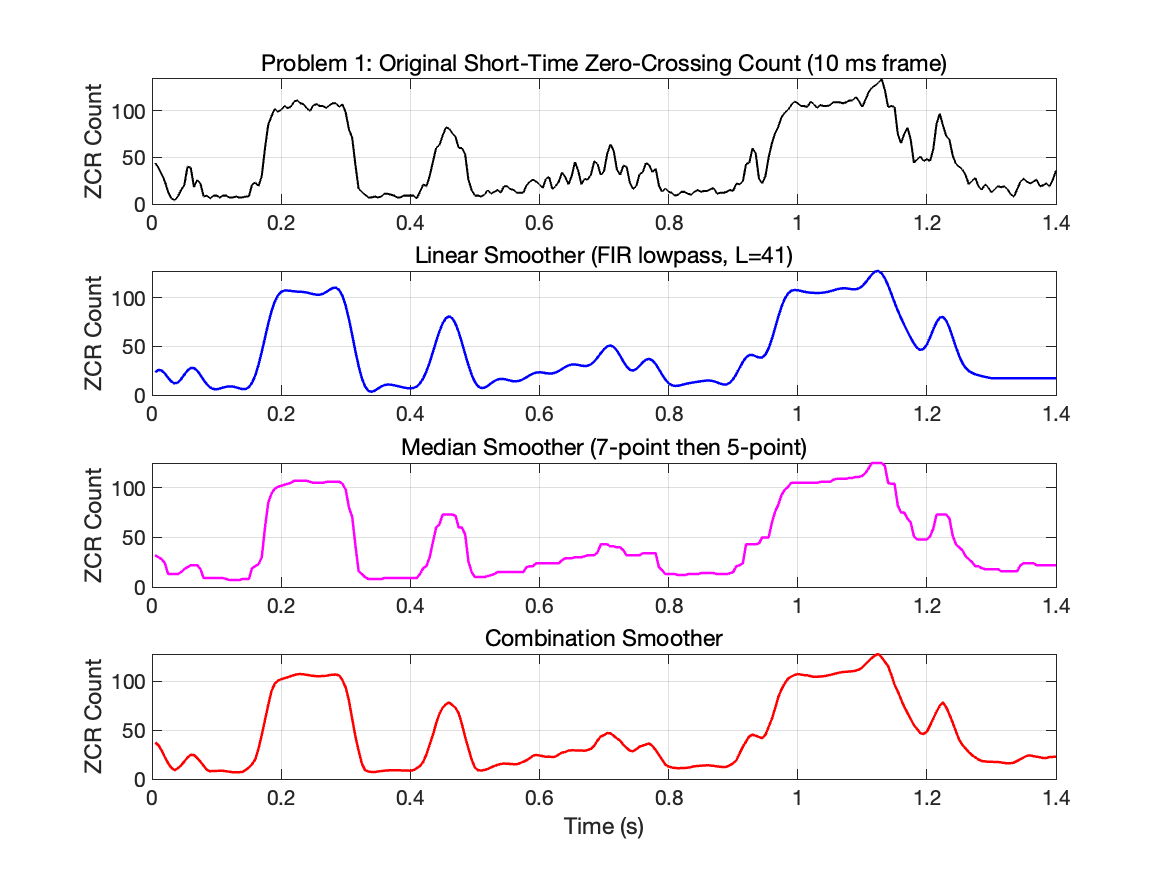
\includegraphics[width=0.96\textwidth]{problem1_zcr_smoothing.png}
    \caption{Problem 1：原始过零率与三类平滑结果}
\end{figure}

为量化平滑效果，计算序列一阶差分标准差（反映局部抖动强度）：
\begin{table}[H]
    \centering
    \caption{Problem 1 指标对比}
    \begin{tabular}{lcc}
        \toprule
        曲线 & 序列标准差 & 一阶差分标准差 \\
        \midrule
        原始 ZCR & 37.6623 & 8.3837 \\
        线性平滑 & 37.3306 & 4.8228 \\
        中值平滑 & 36.9726 & 5.7354 \\
        组合平滑 & 37.0091 & 4.7034 \\
        \bottomrule
    \end{tabular}
\end{table}

可见三种平滑均显著降低了高频抖动，而总体动态范围（序列标准差）变化较小。组合平滑的一阶差分标准差最低，说明其在保留轮廓趋势同时对局部毛刺抑制最强。

\section{Problem 2：基于改进自相关的基音检测}
\subsection{题目要求解读}
题目要求实现基于改进自相关的基音检测流程，核心步骤包括：
\begin{enumerate}
    \item 重采样到 $f_{s\_out}=\SI{10}{kHz}$；
    \item 设计带通滤波器（抑制直流、低频工频干扰及高频噪声）；
    \item 帧长 $L=400$、帧移 $R=100$ 做分帧；
    \item 在 $\mathrm{pdlow}$ 到 $\mathrm{pdhigh}$ 的时延范围内搜索相关峰，得到候选基音周期与置信度；
    \item 对置信度取对数并按 $0.75\times\max$ 设阈值，低于阈值的周期置零；
    \item 对基音周期与置信度做 5 点中值平滑；
    \item 比较原始语音与带通语音的结果。
\end{enumerate}

本实验设定说话人为男性，对应搜索区间：
\begin{equation}
\mathrm{pdlow}=\left\lceil\frac{f_{s\_out}}{200}\right\rceil,\quad
\mathrm{pdhigh}=\left\lfloor\frac{f_{s\_out}}{75}\right\rfloor.
\end{equation}

\subsection{方法实现说明}
对每一帧，计算窗口化信号与延迟信号之间的改进相关：
\begin{equation}
    c(\tau)=\sum_{n=0}^{L-1}x_1[n]\,x_2[n+\tau],\quad \tau\in[\mathrm{pdlow},\mathrm{pdhigh}].
\end{equation}
取最大值位置为基音周期估计，最大值为置信度分数。之后执行对数阈值抑制与中值平滑。

\subsection{结果与分析}
\begin{figure}[H]
    \centering
    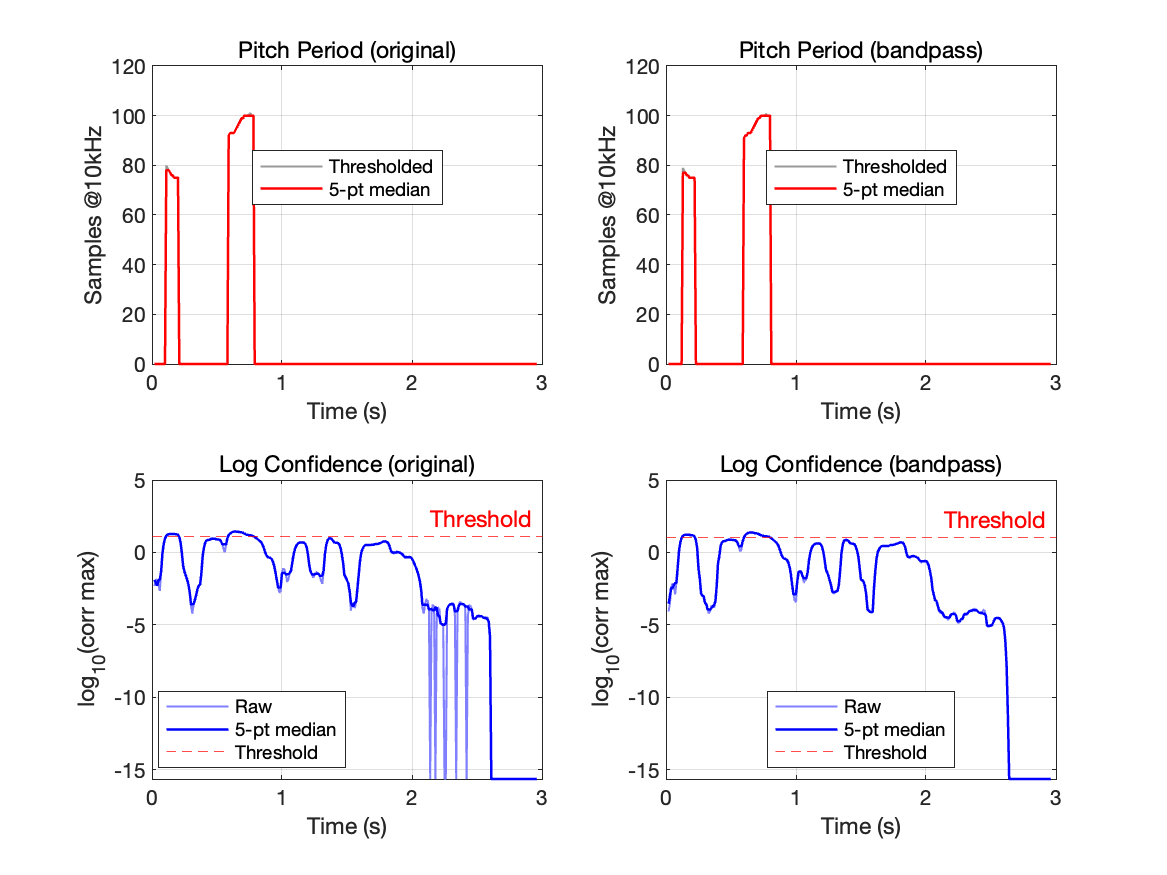
\includegraphics[width=0.95\textwidth]{problem2_autoc_pitch.png}
    \caption{Problem 2：自相关法基音周期与对数置信度}
\end{figure}

\begin{table}[H]
    \centering
    \caption{Problem 2 关键统计量}
    \resizebox{\textwidth}{!}{
    \begin{tabular}{lcccccc}
        \toprule
        信号 & 帧数 & 非零基音帧数 & 占比 & 阈值 & 平均周期(样本) & 平均基频(Hz) \\
        \midrule
        原始语音（s6） & 295 & 30 & 0.1017 & 1.0846 & 90.17 & 110.91 \\
        带通语音（s6） & 295 & 31 & 0.1051 & 1.0313 & 90.00 & 111.11 \\
        \bottomrule
    \end{tabular}}
\end{table}

结果显示原始分支与带通分支的平均周期和平均基频高度一致（约 \SI{111}{Hz}），说明自相关法在该语料上的主周期估计具有较好稳定性。带通后阈值略有下降，非零基音帧数由 30 帧增至 31 帧，提示适度频带约束有助于提升部分边缘帧的可检测性，但总体提升幅度有限。

\section{Problem 3：基于实倒谱的基音检测}
\subsection{题目要求解读}
题目要求使用实倒谱进行基音估计，并引入“主峰/次峰比”来定义高置信区域，步骤重点包括：
\begin{itemize}
    \item 设定 $\texttt{nfft}=4000$；
    \item 在指定倒谱区间 $n\in[n_{\text{low}},n_{\text{high}}]$ 搜索主峰和次峰；
    \item 以比值阈值 $\texttt{pthr1}=4$ 提取可靠帧；
    \item 以边界帧为参考，向相邻帧扩展：若候选周期（主峰或次峰）与边界周期相对偏差不超过 $\pm10\%$，则纳入当前可靠区；
    \item 对得到的周期曲线和置信度曲线进行 5 点中值平滑并绘图。
\end{itemize}

本实验男性参数为：$n_{\text{low}}=40,\ n_{\text{high}}=167$。

\subsection{方法与公式}
实倒谱定义为
\begin{equation}
    c[n]=\mathcal{F}^{-1}\left\{\log\left|X[k]\right|\right\},
\end{equation}
在搜索区间内取主峰位置 $pd_1$ 与次峰位置 $pd_2$，峰值分别为 $p_1,p_2$。若
\begin{equation}
    \frac{p_1}{p_2}\ge p_{\mathrm{thr1}}(=4),
\end{equation}
则该帧视为高置信种子帧。随后执行邻域连续性扩展与中值平滑。

\subsection{结果与分析}
\begin{figure}[H]
    \centering
    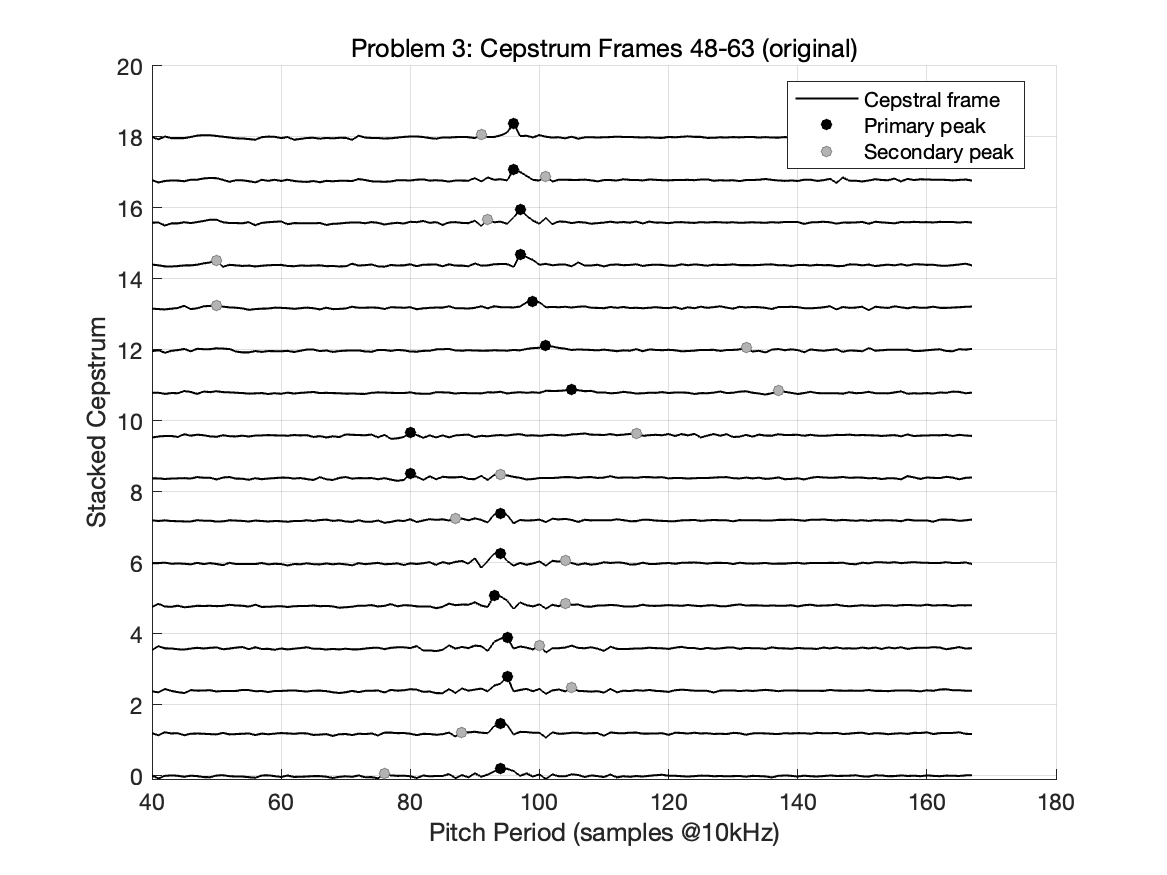
\includegraphics[width=0.92\textwidth]{problem3_cepstrum_waterfall.png}
    \caption{Problem 3：倒谱帧瀑布图（主峰与次峰标注）}
\end{figure}

\begin{figure}[H]
    \centering
    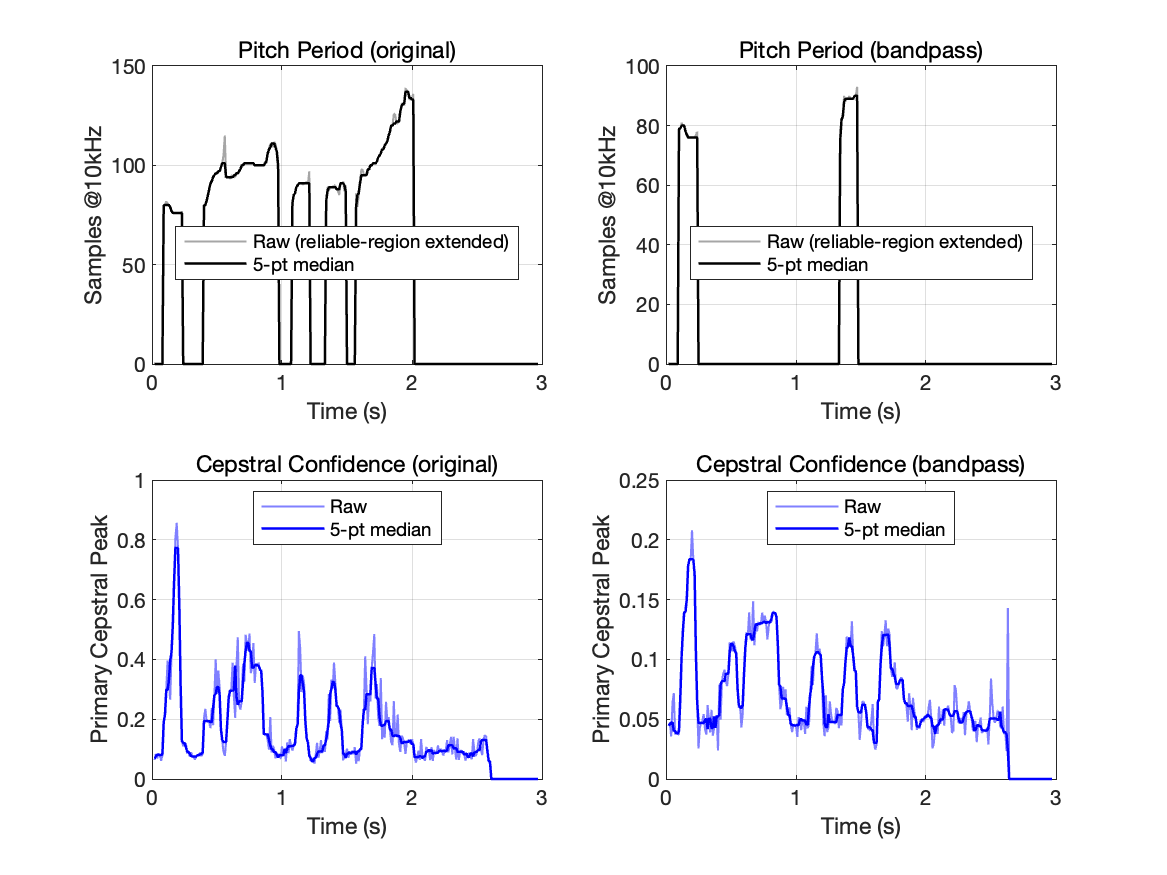
\includegraphics[width=0.95\textwidth]{problem3_cepstrum_pitch.png}
    \caption{Problem 3：倒谱法基音周期与置信度（原始/带通）}
\end{figure}

\begin{table}[H]
    \centering
    \caption{Problem 3 关键统计量}
    \resizebox{\textwidth}{!}{
    \begin{tabular}{lcccccc}
        \toprule
        信号 & 帧数 & 非零基音帧数 & 占比 & 可靠种子帧数 & 平均周期(样本) & 平均基频(Hz) \\
        \midrule
        原始语音（s6） & 296 & 148 & 0.5000 & 58 & 98.34 & 101.68 \\
        带通语音（s6） & 296 & 29 & 0.0980 & 7 & 82.14 & 121.75 \\
        \bottomrule
    \end{tabular}}
\end{table}

从结果看，倒谱法在原始语音上可形成较长的连续有效区段；带通分支的有效帧与可靠种子帧明显减少，但仍可检测出若干稳定片段。该现象表明：倒谱法对谱包络形态与峰值对比度敏感，固定阈值（$p_{\mathrm{thr1}}=4$）在不同预处理链路下的适配性存在差异。为提高跨条件稳健性，建议在后续工作中引入阈值自适应策略，并联合优化带通频带与峰值筛选规则。

\section{结论}
本文完整实现并验证了实验八三项任务。主要结论如下：
\begin{enumerate}
    \item 三类平滑器均有效降低短时过零率抖动，其中组合平滑效果最佳。
    \item 自相关基音检测在原始和带通信号上结果稳定，平均基频基本一致。
    \item 倒谱基音检测在当前语料下对预处理与阈值更敏感，原始语音分支明显优于带通语音分支。
\end{enumerate}

总体而言，本实验验证了“平滑策略 + 置信度控制”在语音参数估计中的关键作用，也体现了不同基音估计方法在鲁棒性与参数敏感性方面的差异。

\end{document}
